The R5 update of Higgs boson cross-section predictions brings together many
theoretical advances made since YR4. The update modifies both the central
values and the uncertainties of the predictions with respect to the YR4.
Figure~\ref{fig:central_values} shows that the central values of the R5
predictions are consistent with those of YR4, within the YR4 uncertainties. Figure~\ref{fig:R5_uncertainties_breakdown} shows
the contributions of the various sources of theoretical uncertainty to the
total relative uncertainty for each production mode. The dominant
uncertainties generally arise from PDF-related sources
(PDF+$\alpha_s$, and PDF$-$TH for ggF) or from QCD scale variation.
Figure~\ref{fig:YR5_ggfsummary_uncertainties} illustrates the change in the
individual uncertainties on ggF since the YR4. Several sources of uncertainty
have been eliminated completely or reduced, while others, namely PDF$-$TH
and QCD scale, have increased for the reasons described in
Section~\ref{sec:ggf_yr4}.

\begin{figure}[!htbp]
    \centering
    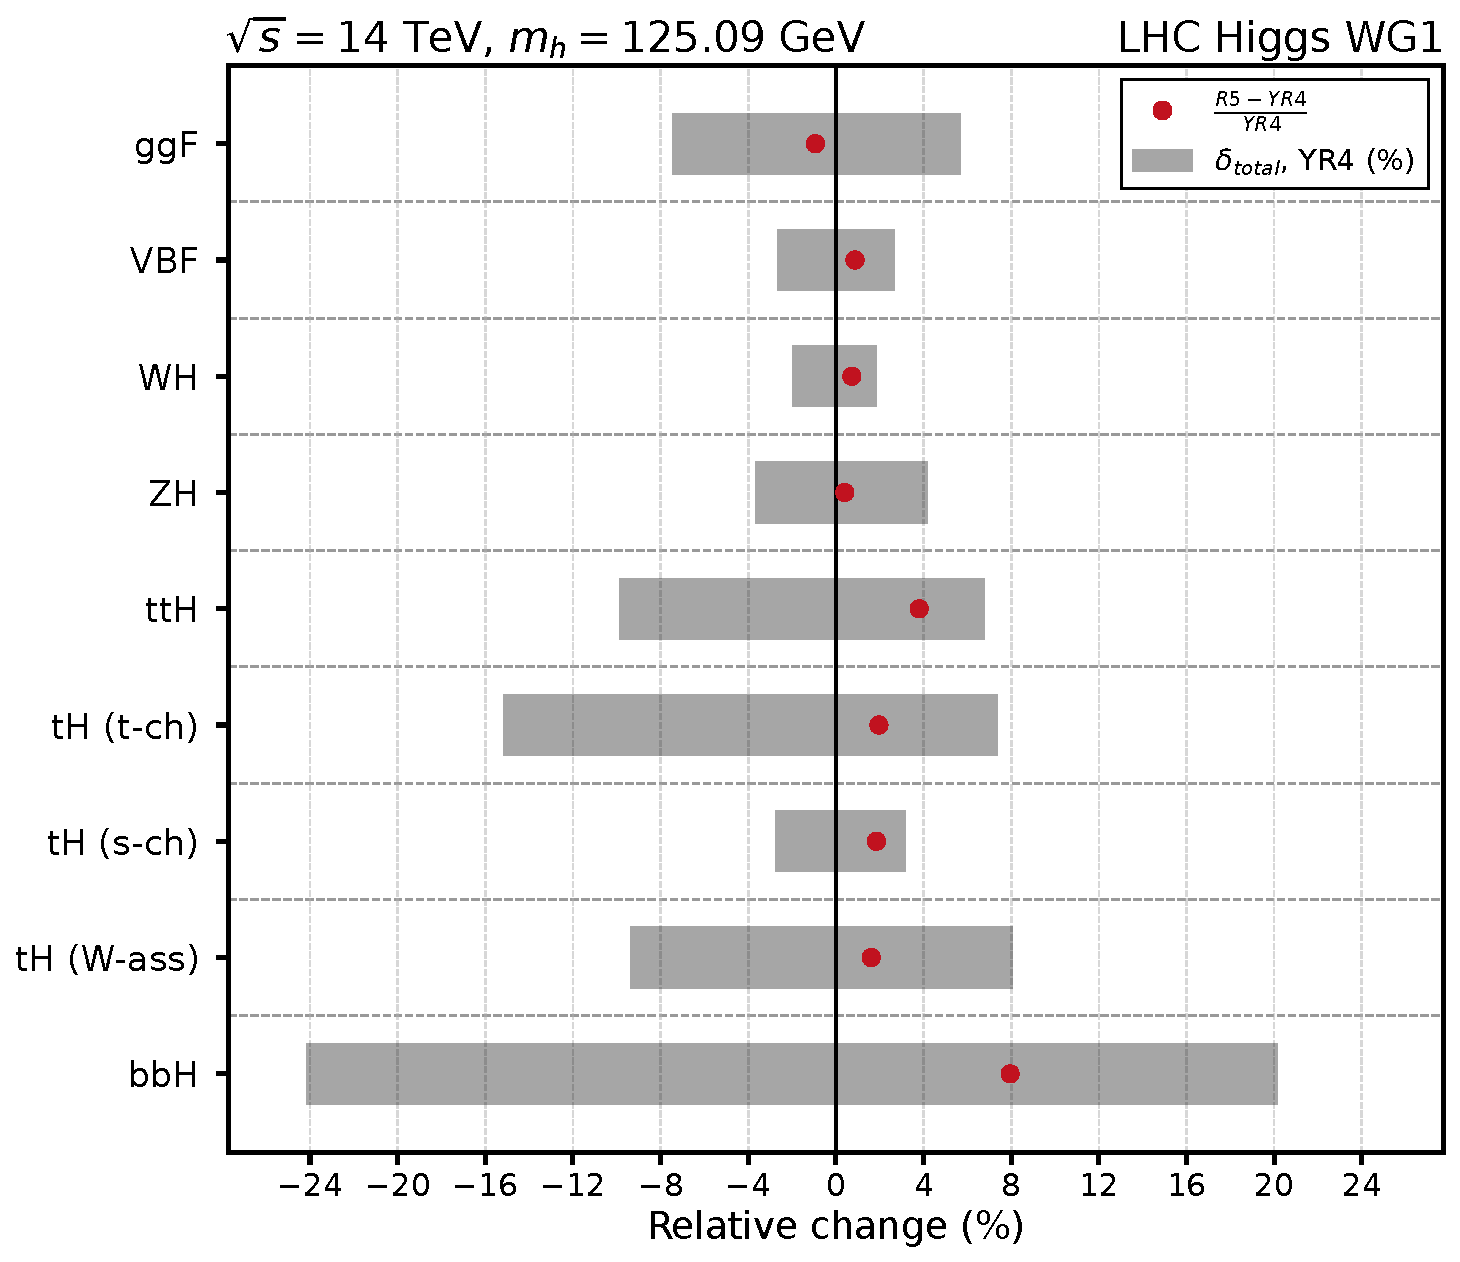
\includegraphics[width=0.95\textwidth]{plots/central_value_comparison.pdf}
    \caption{Change in the central value of the predictions of Higgs boson production cross-sections between the YR4 and R5, relative to the YR4 prediction, for collider energy $\sqrt{s} = 14$ TeV and Higgs boson mass $m_h = 125.09$ GeV. The relative uncertainty on the YR4 prediction is also shown. YR4 predictions for W-associated $tH$ production only exist for $m_h = 125.0$ GeV, so that Higgs mass is used instead.}
    \label{fig:central_values}
\end{figure}

\begin{figure}[!htbp]
    \centering
    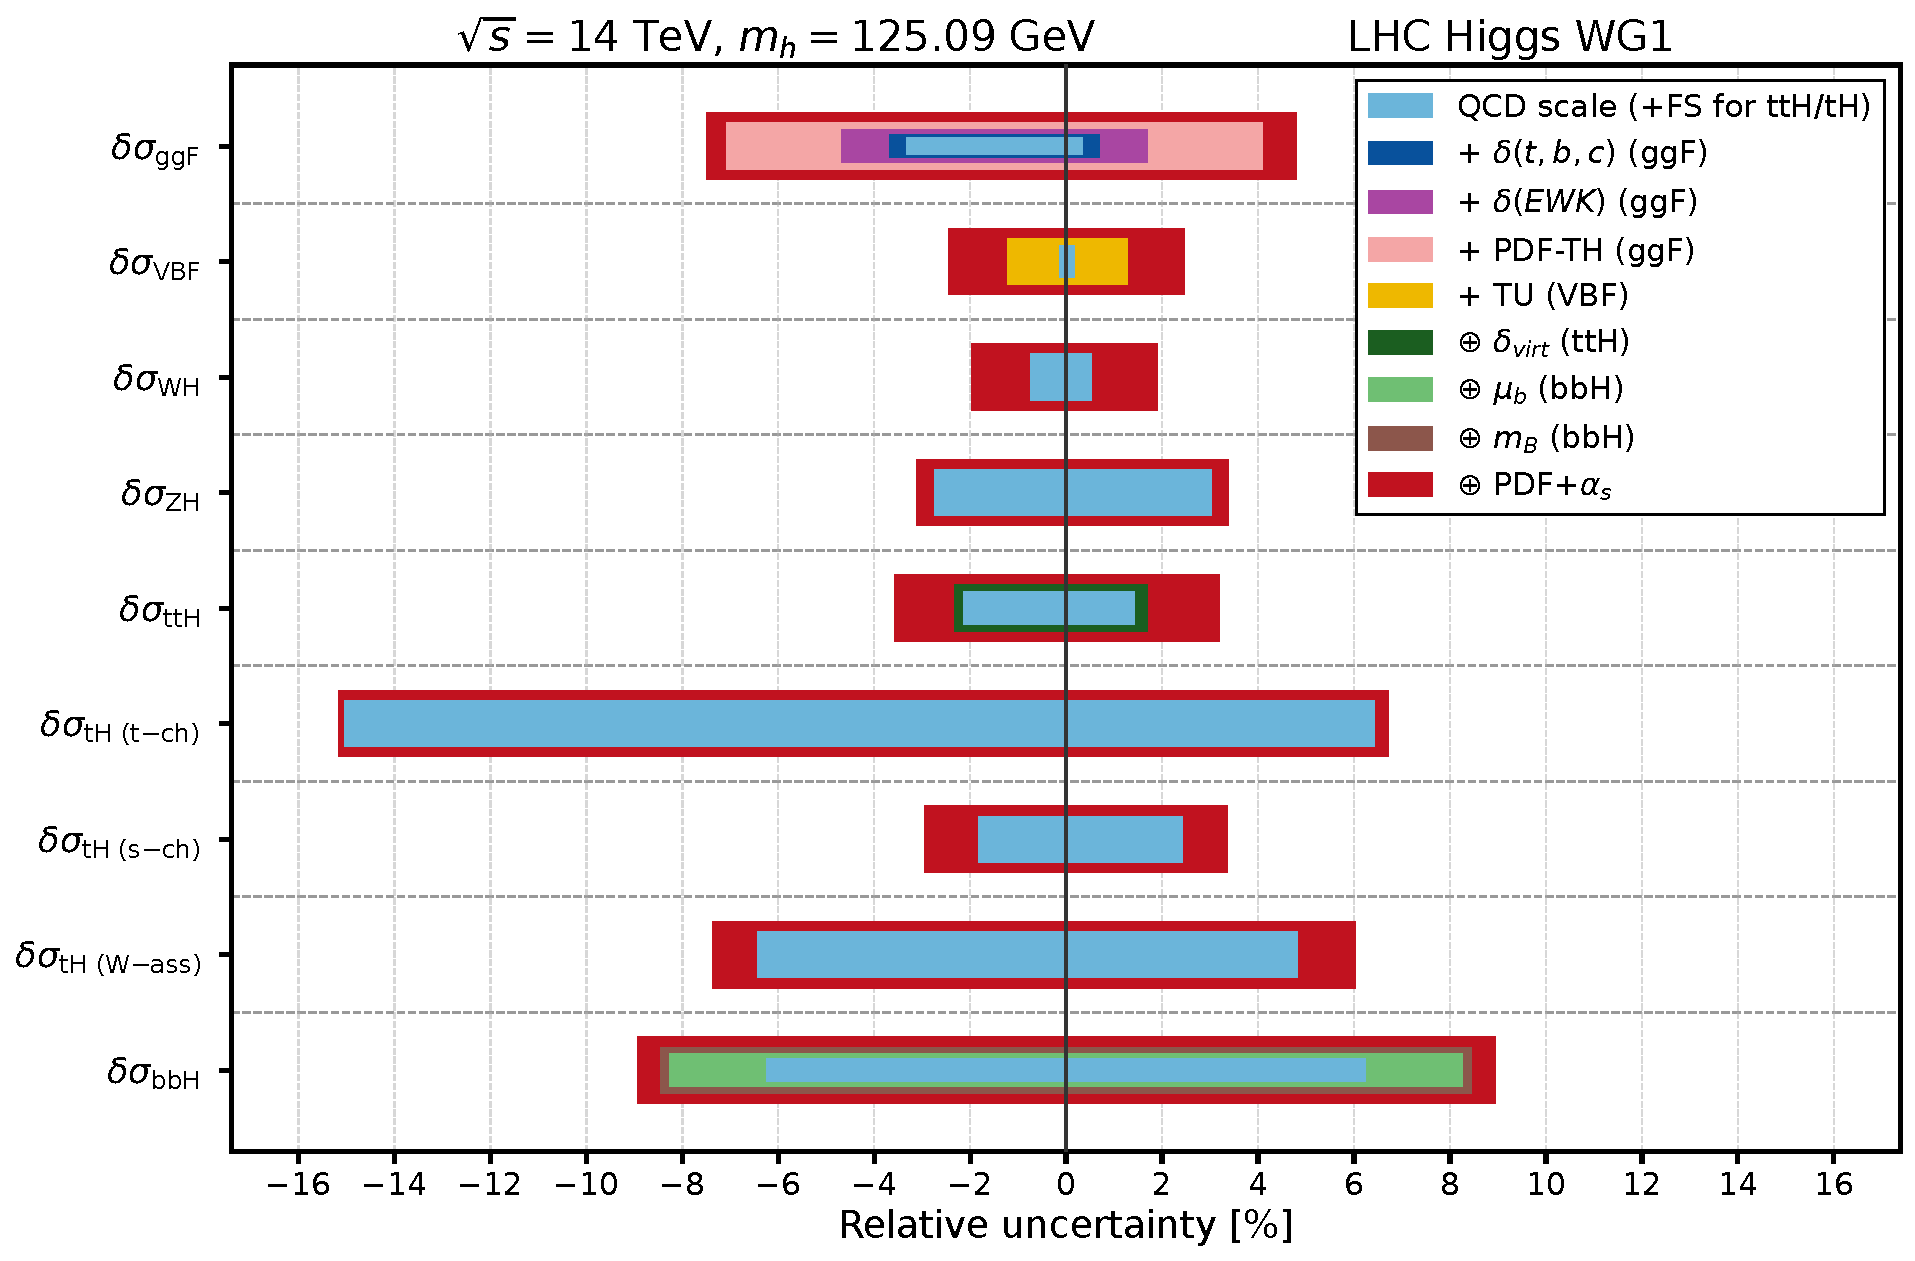
\includegraphics[width=0.95\textwidth]{plots/uncertainty_breakdown_all.pdf}
    \caption{Contribution of various theoretical uncertainties on the Higgs boson production cross sections recommended in this report to the total relative uncertainty. The uncertainties are added one-at-a-time, and the various bars show the total uncertainty after adding each contribution. The symbols in the legend indicate where the source of uncertainty is added linearly ($+$) or in quadrature ($\oplus$).}
    \label{fig:R5_uncertainties_breakdown}
\end{figure}

\begin{figure}[!htbp]
    \centering
    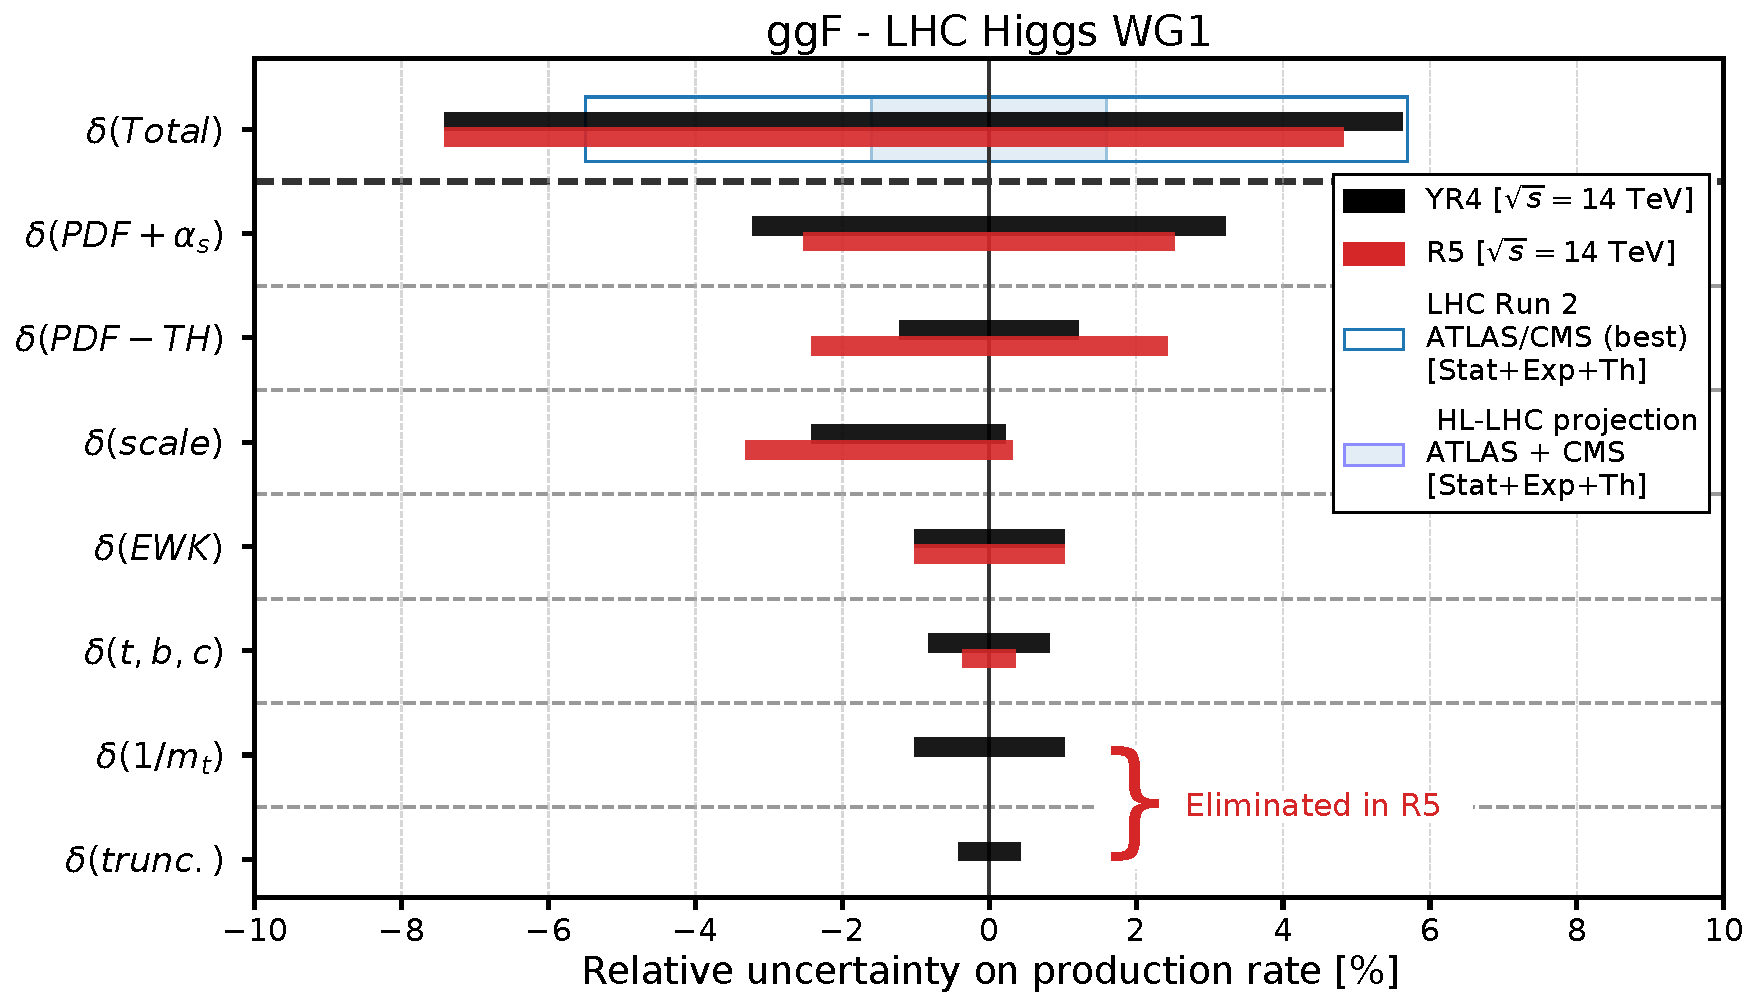
\includegraphics[width=0.95\textwidth]{plots/ggF_uncertainties.pdf}
    \caption{Comparison of the individual contributions to the total theoretical uncertainty on the ggF Higgs boson production cross section recommended in YR4 (black) and in R5 (red). This is compared with the most precise LHC Run 2 Higgs boson signal strength measurement (blue outlined box), whose total uncertainty includes statistical, experimental, and theoretical components, and with the projected HL-LHC ATLAS+CMS combined precision (filled blue box).}
    \label{fig:YR5_ggfsummary_uncertainties}
\end{figure}

Figure~\ref{fig:YR5_summary_uncertainties} expands this comparison by
illustrating the evolution of the theoretical uncertainties on the Higgs
boson production cross-sections between the YR4 and R5 for all production
modes, and compares these results to the precision of measurements of the
Higgs boson production cross-sections at the LHC in Run 2
\cite{ATLAS:2025qxq,CMS:2026nce} and the projected precision of these
measurements at the HL-LHC~\cite{ATLAS:2022hsp}. The corresponding numerical
values are summarised in Table~\ref{tab:prod_uncertainties}. For the ggF,
VBF, ZH and $t\bar t H$ production modes, the anticipated precision of the
measurement at the HL-LHC approaches or exceeds the YR4 theory
precision, illustrating the need for the R5 cross-section update. With the
improved precision of the R5 cross-section predictions, only for ggF does the
projected HL-LHC measurement precision exceed that of the inclusive theory
prediction. Were the optional PDF-theory uncertainty discussed in
Section~\ref{sec:vbf_an3lo} to be included for VBF, bringing its total to
approximately $\pm3.3\%$, the same would become true of VBF. Overall, this
comparison makes clear that the theoretical
advancements brought together in the R5 cross-section predictions are
important for fully exploiting the potential of the HL-LHC. It should also
be noted that the HL-LHC projections themselves assume a reduction by a
factor of two, relative to the YR4, of the theory uncertainties entering the
measurement uncertainty.

Figure~\ref{fig:YR5_summary_uncertainties} also makes clear that the
predictions for most production modes have seen an improvement in theory
precision. For several production modes, the relative uncertainty is reduced
by multiple percentage points; for others, the improvement is more moderate.
It should be noted that for \bbH{}, where the figure shows the largest change
in relative uncertainty, the comparison is made to the YR4 numbers that use
Santander matching, rather than to the updated numbers using
\nlonnllpart{} matching that were released very shortly after the YR4 and
have substantially smaller uncertainties. For all production modes, the
improved precision reflects advances in higher-order calculations,
improvements in PDFs, and refined treatments of theoretical and parametric
uncertainties. To illustrate the potential impact of further improvements in
PDFs, the theory precision without PDF-related uncertainties is also shown
in the figure. For several of the most precisely predicted production modes,
this results in a substantial reduction of the total uncertainty,
demonstrating that PDF-related uncertainties are an important limitation and
that further progress in this area will be crucial ahead of the HL-LHC.

\begin{figure}[!htbp]
    \centering
    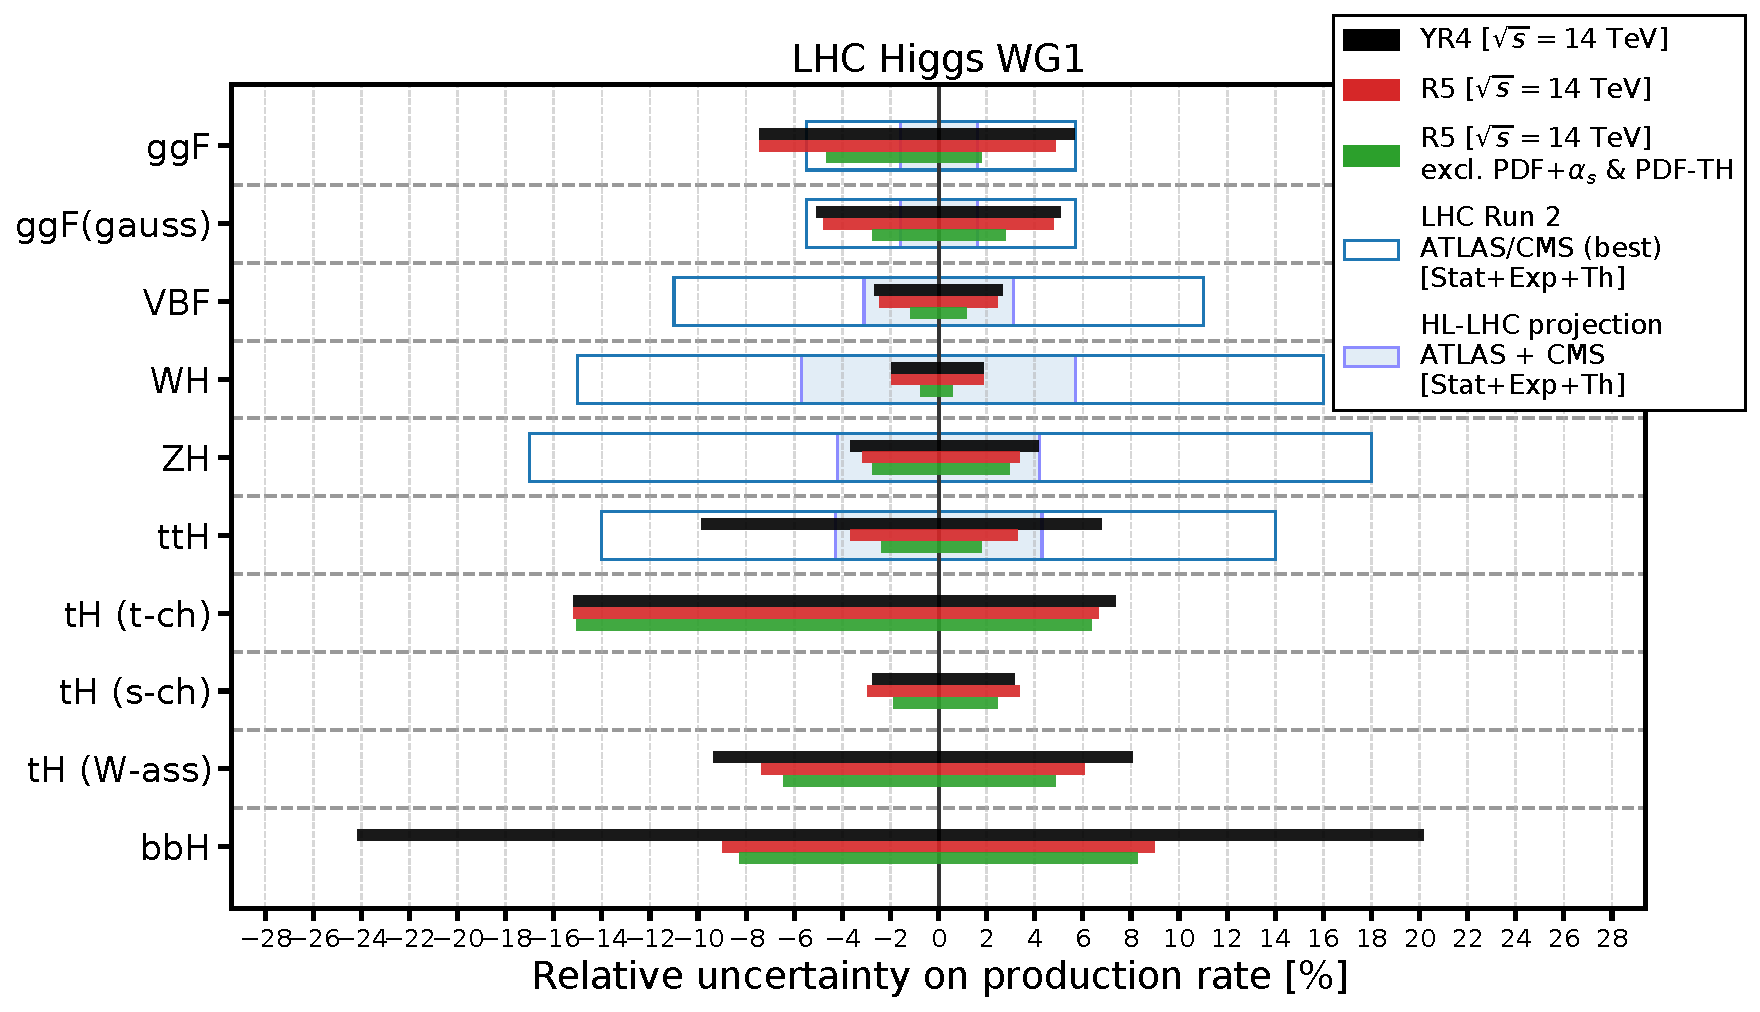
\includegraphics[width=0.95\textwidth]{plots/production_mode_uncertainties.pdf}
    \caption{Comparison of the theoretical uncertainties on the Higgs boson production cross sections recommended in YR4 (black) and in R5 (red) for collider energy $\sqrt{s} = 14$ TeV and Higgs boson mass $m_h = 125.09$ GeV. The current recommendations excluding the PDF$+\alpha_{s}$ and PDF$-$TH contributions are also shown (green). These are compared with the most precise LHC Run 2 Higgs boson signal strength measurements (blue outlined boxes), whose total uncertainties include statistical, experimental, and theoretical components, and with the projected HL-LHC ATLAS+CMS combined precision (filled blue box).}
    \label{fig:YR5_summary_uncertainties}
\end{figure}

\begin{table}[htbp]
\renewcommand{\arraystretch}{1.3}
\setlength{\belowcaptionskip}{10pt}
\centering
\caption{Relative uncertainties (\%) on Higgs boson production cross sections from YR4 and R5, including the R5 uncertainties excluding PDF$+\alpha_{s}$ and PDF$-$TH contributions. These are compared with the most precise LHC Run~2 Higgs boson measurements from ATLAS and CMS, whose total uncertainties include statistical, experimental, and theoretical components, and with the projected HL-LHC ATLAS+CMS combined precision. For the Run~2 measurements and HL-LHC projections, \bbH{} is grouped with ggF and the $tH$ channels are not considered separately, so they are not shown.}
\label{tab:prod_uncertainties}
\begin{tabular}{lccccc}
\toprule
Production mode &
YR4 &
R5 &
R5 (no PDF) &
Run 2 &
HL-LHC \\
\midrule
ggF          & ${}^{+5.6}_{-7.4}$  & ${}^{+4.8}_{-7.4}$  & ${}^{+1.7}_{-4.6}$  & $\pm5.8$           & $\pm1.6$ \\
VBF          & $\pm2.6$            & $\pm2.4$            & $\pm1.1$            & ${}^{+11.7}_{-10.7}$& $\pm3.1$ \\
WH           & ${}^{+1.8}_{-1.9}$  & ${}^{+1.8}_{-1.9}$  & ${}^{+0.5}_{-0.7}$  & $\pm15.6$           & $\pm5.7$ \\
ZH           & ${}^{+4.1}_{-3.6}$  & ${}^{+3.3}_{-3.1}$  & ${}^{+2.9}_{-2.7}$  & ${}^{+17.0}_{-15.6}$& $\pm4.2$ \\
ttH          & ${}^{+6.7}_{-9.8}$  & ${}^{+3.2}_{-3.6}$  & ${}^{+1.7}_{-2.3}$  & ${}^{+23.4}_{-19.4}$& $\pm4.3$ \\
tH ($t$-ch.) & ${}^{+7.3}_{-15.1}$ & ${}^{+6.6}_{-15.1}$ & ${}^{+6.3}_{-15.0}$ & --                  & -- \\
tH ($s$-ch.) & ${}^{+3.1}_{-2.7}$  & ${}^{+3.3}_{-2.9}$  & ${}^{+2.4}_{-1.8}$  & --                  & -- \\
tH ($W$-as)  & ${}^{+8.0}_{-9.3}$  & ${}^{+6.0}_{-7.3}$  & ${}^{+4.8}_{-6.4}$  & --                  & -- \\
bbH          & ${}^{+20.1}_{-24.1}$& ${}^{+8.9}_{-8.9}$  & ${}^{+8.2}_{-8.2}$  & --                  & -- \\
\bottomrule
\end{tabular}
\end{table}

Looking beyond the present recommendations, continued progress in PDF
determinations will be particularly important. Approximate N$^3$LO PDF sets
are already available, and the perturbative ingredients entering N$^3$LO
evolution and matching continue to improve, as discussed in
Section~\ref{sec:an3lo-pdfs}. Establishing a robust common prescription for
PDFs at this accuracy will be important for processes whose hard-scattering
cross sections are already known at N$^3$LO. At the same time, as
percent-level precision becomes increasingly relevant, a more uniform
treatment of QED evolution and photon-initiated contributions will become
desirable. Further progress in higher-order perturbative calculations and
in the assessment of process-specific residual theoretical uncertainties
will remain important for production modes where these effects continue to
limit the prediction.

The recommendations presented in this report represent the current state of
the art. Continued progress in higher-order perturbative calculations, PDF
determinations, and the assessment of residual theoretical uncertainties
will be essential to match the experimental precision expected from the
HL-LHC programme.

